%Du begynder bare at skrive
\chapter{Astrofysik}
\section{Kosmologi}
Kosmologi er læren om universets skabelse, udvikling og endeligt. Når vi snakker om universets størrelse, er det normalt det synlige univers, vi mener. Dette er den del af universet, hvor lys har nået hen til os, så vi kan observere det. Længere ude er informationen ikke nået frem til os endnu, så vi ved ikke hvor stort hele universet er. 

Det passer med \textbf{det kosmologiske princip}. Ifølge dette er universets love og konstanter ens overalt og massen er ligevægt fordelt (set fra en stor nok skala). Det kan deles op i to postulater: Universet er homogent (ens i hvert område) og isotropt (ser ens ud, uanset hvilken retning man kigger i), som illustreret i figur \ref{isohomo}. Det kosmologiske princip behøver ikke gælde, men vi har ikke observeret noget der bryder med det. Så normalt antager vi, det gælder, da det er det simpleste - vi har ingen grund til at tro universets egenskaber pludselig ændrer sig et sted. Det er en god approksimation på skalaer fra 200 Mpc (megaparsec) og opefter. 1 pc er cirka 3 lysår, så det er $3*10^8$ lysår. På små skalaer holder det selvfølgelig ikke. For eksempel er du tættere end luften omkring dig og Solen kan udpege en særlig retning inden for solsystemet.

Antagelsen om at vores Univers er homogent og isotropt, er understøttet af
kortlægningen af den kosmiske mikrobølgebaggrund (eng: CMB – cosmic microwave
background). Baggrunden består af stråling fra det tidspunkt, hvor Universet blev
gennemsigtigt (ca. 380 000 år efter Big Bang) – altså hvor temperaturen af plasmaet
og strålingen dannet efter Big Bang faldt tilstrækkeligt til, at frie elektroner kunne
kombinere med atomkerner og danne hydrogen og helium (af historiske årsager
kaldes dette for rekombinationen, men man kalder det også for foton-afkoblingen)
og lyset kunne undslippe. Den kosmiske mikrobølgebaggrund er derfor det ældste
lys i Universet! Dengang var strålingen i UV-området, men udvidelsen af Universet
(se næste sektion) har nu kølet den til en temperatur på 2.73 K og flyttet den til mikrobølgeområdet. Den kosmiske mikrobølgebaggrund er blevet kortlagt af flere
missioner, først COBE (COsmic Background Explorer), siden WMAP (Wilkinson
Microwave Anisotropy Probe) og senest Planck, se figur \ref{CMB}. Det ses, at selv med høj opløsning er kortet uniformt – beviset på et næsten
homogent og isotropt tidligt Univers. Men små fluktuationer i tætheden er stadig til
stede, og var det ikke for disse, ville den gravitationelle tiltrækning ikke have kunnet
skabt de galakser vi observerer (og bebor!) idag.

\begin{figure}[h]
	\centering
	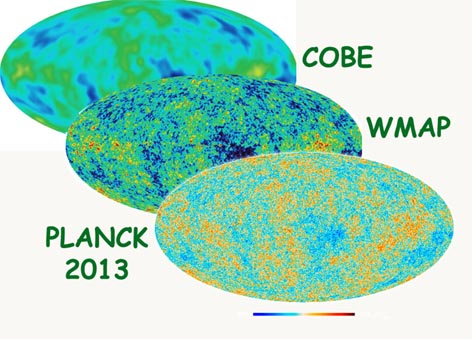
\includegraphics[width=0.7\textwidth]{Astrofysik/Astrofig/CMB.jpg}
	\caption{Kortlægningen af den kosmiske mikrobølgebaggrund af COBE, WMAP og
		Planck. Mælkevejen, som ellers ville være til stede i billedet, er redigeret ud. Fra http:
		//www.planetastronomy.com/astronews/astrn-2013/04/astron3.jpg}
	\label{CMB}
\end{figure}

\begin{figure}[h]
	\centering
	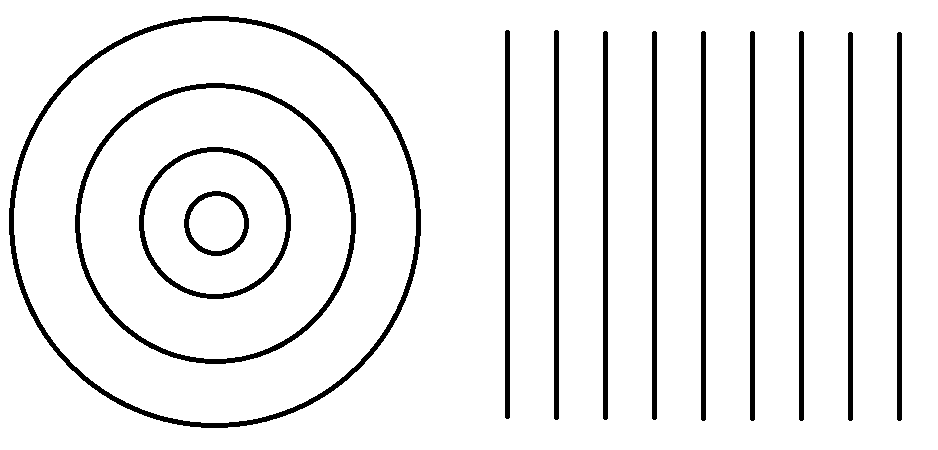
\includegraphics[width=0.7\textwidth]{Astrofysik/Astrofig/isohomo.png}
	\caption{Venstre: Illustration af isotropi. Fra midten ser verden ens ud i alle retninger. Højre: Illustration af homogenitet. Kigger man på et stort nok udsnit af verden, vil det se ud som alle andre udsnit.}
	\label{isohomo}
\end{figure}

\s
Afstand er et vigtigt begreb i astrofysikken og kosmologien. En af de mest brugte metoder til bestemmelse af afstande er gennem et objekts \textit{luminositet}. Et objekts absolutte luminositet $L$ er defineret som den energi, der er udsendt per sekund. Det har vist sig, at en stjernes luminositet, hvis vi antager, at det er et sortlegeme, er relateret til dets radius $R$ og temperatur $T$:
\begin{equation}
L = 4\pi\sigma R^2T^4 \propto R^2 T^4
\end{equation}
hvor $\sigma$ er Stefan-Boltzmann's konstant. \\
Hvis denne energi er udsendt uniform i alle retning og modtages i en afstand $d_L$ væk, er den modtagede \textit{tilsyneladende luminositet} - eller \textit{flux} - givet ved:
\begin{equation}
f = \frac{L}{4\pi d_L}.
\end{equation}
Her er $d_L$ luminositetsafstanden. Indenfor astronomiens verden beskrives et objekts lysstyrke ved \textit{magnitudesystemet}. Dette er et logaritmisk system, der rækker helt tilbage til Hipparchos i antikkens Grækenland. Af historiske årsager fungerer systemet således, at jo højere magnitude, desto svagere ser objektet ud på himlen og omvendt. Dengang fandtes der ikke teleskoper, som i dag, så alle målinger af stjerne blev taget per øjemål. Dengang gik skalaen fra 0 til og mg med 6, hvor 0 var det stærkeste på himlen og så fremdeles.

\subsection{Standard candles}

Et standard candles er et astronomisk objekt der har en kendt absolut magnitude. Disse er super vigtige for astronomer, da man ved hjælp af den tilsyneladende magnitude af et objekt kan bestemme afstanden ved at bruge:
\begin{equation}
m-M=5\cdot \log(d) - 5 ,
\end{equation}
hvor $m$ er den tilsyneladende magnitude (den lysstyrke vi ville se fra Jordens overflade), $M$ er den absolutte magnitude (den faktisk lysstyrke af et objekt), og $d$ er afstanden til objektet målt i parsec.

De mest anvendte standard candles indenfor astronomi er Cepheide variable stjerner og RR Lyræ stjerner. I begge tilfælde kan stjernes absolutte magnitude bestemmes ud fra deres variabilitetsperiode.

Den nye dreng i klassen er Type Ia supernovaer. Disse kan også klassificeres som standard candles, men er i virkeligheden standardiserbar candles, da de ikke har præcist den samme maksimale lysstyrke. Forskellene i deres maksimale lysstyrke er imidlertid korreleret med, hvor hurtigt lyskurven aftager efter maksimal lysstyrke. Her ser man på differencen mellem den maksimale lysstyrke og lysstyrken 15 dage efter. Dette kaldes også $\Delta~m_{15}$. Hvis denne har en værdi mindre end $1$ er objektet lysstærkt, mens den ved en værdi over $1$ er lyssvag.

\section{Big Bang og CMB}

\subsection{Rødforskydning}
\subsubsection{Dopplerforskydning}
Du kender nok til, at hvis en ambulance kører forbi, så lyder sirenens tone højere når den nærmer sig, og dybere når den kører væk. Det kalder vi \textbf{Dopplerforskydning}. %Find gerne lydklip til undervisningen
Dette er fordi lydbølgerne skubbes sammen og strækkes, afhængigt af hvilken fart de udsendes med i forhold til lytteren. Hvis en ambulance kører mod dig, og du står stille, vil du høre bølgerne sammenpresset. Men hvis du selv kører med samme hastighed foran ambulancen, så vil du høre dem på samme måde, som de bliver udsendt - altså på samme måde som hvis begge biler stod stille, da det er den relative hastighed, som er afgørende.

\begin{figure}[h!]
	\centering
	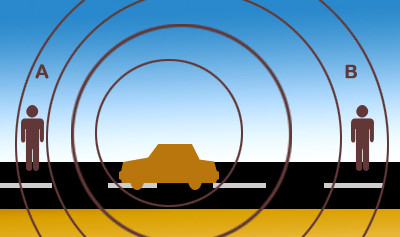
\includegraphics[width=0.7\textwidth]{Astrofysik/Astrofig/doppler.jpg}
	\caption{Dopplerforskydning af lyden fra en bil, der kører mod venstre. Person A vil høre end højere tone end person B, og personen i bilen vil høre noget et sted derimellem. Ringene viser et fast punkt på lydbølgerne, fx alle bølgetoppe.}
	\label{shapes}
\end{figure}

Det samme sker for lys. Hvis en ambulance kører væk vil både tonen blive dybere og lyset fra den en smule rødere. Bemærk dog at selvom fotoner og lydbølger har højere energi ved korte bølgelængder, så mister de ikke energi ved Dopplerforskydning - der er bare sket et skift i perspektivet, man ser bølgerne fra. Fra bølgens eget synspunkt (hvis man følger den) har den samme bølgelængde og energi hele tiden.
\subsubsection{Kosmologisk rødforskydning}
Edwin Hubble opdagede i 1920'erne, at galakser langt borte ser rødforskudte ud, men dette skyldes \underline{ikke} Dopplerforskydning fra galaksernes egenhastighed i forhold til os. Så ville vi have forventet, at lige så mange galakser var rødforskudte som blåforskudte, hvis de starter med en tilfældig hastighed. Og det gør de jo - for hvorfor skulle de have en særlig retning i forhold til os? Det ville bryde med isotropien. 

Hubble opdagede, at galakserne oftere er rødforskudt end blåforskudt, og jo længere væk de er, desto mere rødforskudte er de også. Han formulerede "Hubbles lov", der beskriver den direkte proportionalitet mellem afstand og fart af en galakse:
\begin{align}
v=H_0 D \label{Hubbleslaw}
\end{align}
Her er $v$ farten, $D$ er afstanden til galaksen, og $H_0=67.7\pm0.5$ er Hubbles konstant, som er den nuværende værdi af Hubble-parameteren (der ikke er konstant).

Galaksers relative hastighed til os er altså større, desto længere væk de er. Og sådan vil det se ud fra ethvert punkt i universet. Derfor må rødforskydningen stamme fra at alting bevæger sig længere væk fra hinanden, som rosiner i en hævende bolle. Det er netop, hvad der sker - universets dej dvs. selve rummet "hæver". Galakserne har lige ofte egenhastigheder der går mod os som fra os, men hastigheden, selve rummet udvider sig med, er vigtigere for galakser langt væk. For fjerne galakser skal lyset bevæge sig gennem mere rum for at nå frem til os. Derfor når lyset at blive strukket mere end ved nære galakser. 

Ved rødforskydning fra rummets udvidelse mister lyset rent faktisk energi i modsætning til almindelig Dopplerforskydning. Dette er selvfølgelig et brud på energibevarelse, men det er egentlig ikke et problem, da man ikke kan betragte universet som et lukket system, fordi det udvider sig. Energibevarelse behøver kun gælde i lukkede systemer. Nogle mener dog, at ændringen i energi fra rummets udvidelse (og den mørke energi der opstår, se sektion \ref{bestanddele}) udlignes af at den gravitationelle energi falder til endnu lavere negative niveauer, således at universets totale energi altid er 0.

Måden, man måler rødforskydningen på, er ved at opsplitte lyset i dets forskellige bølgelængder. Dvs. man tage spektrer af fjerne objekter og derefter genkender man mønstre fra jordiske laboratorier. Niels Bohr opdagede at elektroner kun kan eksistere i bestemte baner om atomkernerne, men ikke mellem disse. Hver bane har en bestemt energi, så elektronernes energi i atomer er kvantiseret, dvs. de findes kun i bestemte pakker. Når en elektron henfalder til en lavere tilstand, kommer den af med overskydende energi ved at udsende en foton. Og hvis en foton med passende energi rammer en elektron, kan fotonen blive absorberet, så elektronen kommer op i en højere energitilstand. 

For lysspektrer gælder 3 love kaldet Kirchoffs love (ikke at forveksle med Kirchoffs love for elektriske kredsløb), som er illustreret i figur \ref{kirchoff}
\begin{itemize}
	\item Varme, uigennemsigte objekter udsender lys kontinuert over hele spektret. Ideelt set ville det give spektret for sortlegemestråling, og det er en særligt god approksimation for varme stjerner. Mindre stjernes lys er mere "forurenet" af effekter fra molekylær hydrogen (det er relativt koldt) og andre stoffer.
	\item Varme, gennemsigte gasser udsender lys og danner emissionsspektrer.
	\item Kolde gasser danner absorptionslinjer. Hvis en stjerne ligger bagved og sender lys mod os, vil skyen absorbere lyset og udsende det senere i en tilfældig retning. Det er meget usandsynligt retningen er mod os igen, så vi ser mindre lys ved denne bølgelængde.
\end{itemize}

\begin{figure}[h]
	\centering
	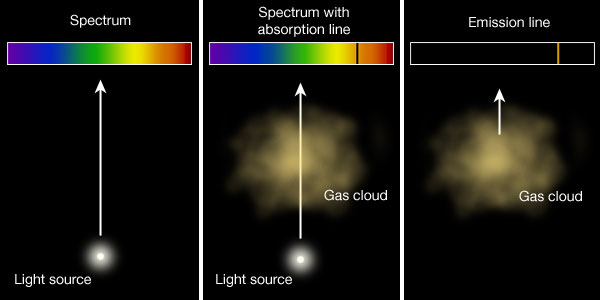
\includegraphics[width=0.7\textwidth]{Astrofysik/Astrofig/kirchoffslaws.jpg}
	\caption{Kontinuert spektrum (til højre), absorptions-spektrum (midtfor) og
		emissions-spektrum (til venstre) fra http://astro.psu.edu/public-outreach/
		fireworks-masks-1/absorption-and-emission-spectra}
	\label{kirchoff}
\end{figure}

Hvis man har galakse med en stjerner, som udsender et bredt spektrum af lys, vil lyset både bevæge sig gennem stjernens ydre "kolde" lag og galaksens gasskyer, før det når os. Stjerner og skyer består af forskellige stoffer såsom hydrogen. Når de belyses, absorberer hydrogenet fotoner med de energier, der svarer til energiforskellen mellem banerne i hydrogen. Der dannes derfor et helt bestemt mønster af absorbtionslinjer i spektret, som er unikt for fx hydrogen. For en rødforskudt galakse vil mønsteret ligge ved længere bølgelængder end det vi måler for hydrogen på Jorden, men det er stadig genkendeligt.

Når vi kan genkende et mønster af absorptionsliner eller emissionslinjer, selvom det ligger forskudt ved andre bølgelængder end normalt, så kan vi finde rødforskydningen. Den er defineret som forskellen mellem observeret bølgelængde $\lambda_{obs}$ og laboratoriebølgelængde $\lambda_{lab}$ i forhold til laboratoriebølgelængden. Det er altså den relative forskydning i forhold til den oprindelige bølge. Lad os opskrive det som

\begin{align}
z=\frac{\lambda_{obs}-\lambda_{lab}}{\lambda_{lab}}.
\end{align}
Rødforskydningen $z$ er relateret til farten $v$ således:
\begin{align}
z+1=\sqrt{\frac{1+\frac{v}{c}}{1-\frac{v}{c}}}
\end{align}
For hastigheder meget langsommere end lysets hastighed i vakuum $c$, kan det forsimples til:
\begin{align}
z\approx\frac{v}{c}
\end{align}

Rødforskydning er altså et form for afstandsmål, men også et tidsmål, da lyset har rejst i lang tid, hvis det har nået at passere en stor afstand og er blevet meget udtrukket. Hvordan rødforskydningen relaterer til andre måder at måle afstand afhænger af hvordan rummet strækker lyset. Og det afgøres af universets form via generel relativitetsteori.

\subsection{Universets form}

Universet har samlet set en form. Vi har 3 tydelige rumdimensioner omkring os, og vi er vant til, at hvis man tegner to parallelle linjer, så vil de aldrig krydse, og en trekant har altid 180 grader. Men dette gælder kun i fladt rum! Forestil dig for eksempel en trekant tegnet på en globus; den vil faktisk have mere end 180 grader. På samme måde vil en trekant tegnet på en saddel have mindre end 180 grader, som på Figur \ref{shapes}. Hvis rummet er kugleformet, har det en positiv krumning, og hvis det er saddelformet, har det en negativ krumning. I fladt rum er krumningen 0.

\begin{figure}[h!]
	\centering
	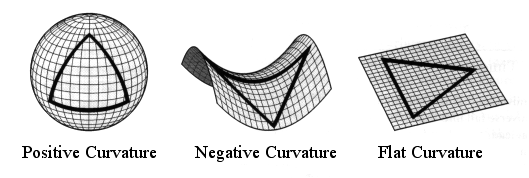
\includegraphics[width=0.7\textwidth]{Astrofysik/Astrofig/universe_geometry.png}
	\caption{Trekanter i forskellige rum har forskellige vinkelsummer. Billede fra http://abyss.uoregon.edu/~js/images/universe\_geometry.gif}
	\label{shapes}
\end{figure}

Hvis et objekt er i frit fald, eller hvis man har en lysstråle, vil de bevæge sig langs en ret linje i rummet. Men hvis selve rummet krummer, så gør den "rette" linje det også. Derfor kan man se rummets krumning ved at kigge på lyset fra objekter langt væk. Den viser sig ved om ting ser forstørrede eller formindskede ud (om strålerne spredes eller samles som i en linse), og disse målinger viser, at rummet er fladt med en præcision på 0.5 \%. Det vender vi tilbage til i sektion \ref{bestanddele}. %Kilde + illustration

Hvis rummet var positivt krumt og småt nok, ville det også betyde at lyset kunne nå hele vejen rundt, og vi ville se de samme objekter flere steder på himlen, hvilket heller ikke er observeret. Så det synlige univers er i hvert fald meget fladt - men måske har rummet en svag krumning, der bare ikke kan ses her. Selvom Danmark ser fladt ud, kan hele jordkloden jo godt være rund.

Hvis rummet er positivt krumt, er det endeligt, mens fladt eller negativt rum kan være uendeligt stort. Det er dog også muligt for rum både at være fx fladt og endeligt, men så bryder man det kosmologiske princip.

Vi kan sammenligne universets størrelse ved forskellige tidspunkter gennem en skalafaktor $a(t)$. Vi definerer den nuværende faktor til 1, $a(t_0)=1$, hvor $t_0$ er nu. Der gælder sammenhængen:
\begin{align}
\frac{a(t_0)}{a(t)}=1+z\\
a(t)=\frac{1}{1+z}
\end{align}
Så man kan let omregne rødforskydning til skalafaktoren, fra dengang lyset blev udsendt.

Som beskrevet % i \ref{Hubble}
i forbindelse med ligning \ref{Hubbleslaw} er Hubblekonstanten ikke konstant, men er blot den nuværende værdi af Hubbleparameteren. Hubbleparameteren er
\begin{align}
H=\frac{v}{D}=\frac{\dot{a}}{a},
\end{align}
hvor en prik som bekendt betyder differentieret mht. tid, så det er den relative ændring i skalafaktoren. Hvis vi sætter det i anden og bruger noget generel relativitetsteori, får vi \textbf{Friedmann-ligningen}:
\begin{align}
H^2=\left(\frac{\dot{a}}{a}\right)^2=\frac{8\pi G \rho}{3}-\frac{\kappa c^2}{a^2}+\frac{\Lambda}{3}
\end{align}
Denne ligning er superinteressant, da den viser os hvordan universet udvikler sig. Det er en andengradsligning med $a$ indeholdende konstanter som gravitationskonstanten $G$ og lysets fart i vakuum $c$. $\kappa$ kan være 1, 0 og -1 og dette afgør krumningen, der som bekendt kan være positiv, 0 eller negativ. $\Lambda$ er den kosmologiske kontant. Uden denne ville rummet trække sig sammen, fordi massen krummer det, så Einstein introducerede $\Lambda$ for at holde universet statisk. Det har han senere kaldt sin største fejl, efter Hubble opdagede universet er dynamisk. Man har dog genintroduceret konstanten for at accelerere udvidelsen, da man opdagede mørk energi i 1998. Lad os se på, hvad det egentlig er.

\subsection{Universets komponenter} \label{bestanddele}
Universets udvikling og skæbne afhænger af dets indhold. Det består af:
\begin{itemize}
	\item Stråling/relativistisk stof: Fotoner og neutrinoer (fordi de har ingen til meget lav masse og høj hastighed)
	\item Stof: Almindeligt stof, antistof og mørkt stof har alle masse, så her kalder jeg dem samlet set "stof". Egenskaben masse afgør, hvor mange kræfter man skal bruge på at accelerere partiklerne, men også hvor meget de krummer rummet omkring sig. 
	\item Kosmologisk konstant: Den form for mørk energi, vi antager universet er fyldt med. Det får universets udvidelse til at accelerere, er ligeligt fordelt overalt og fortyndes ikke fra udvidelsen.
\end{itemize}

Disse komponenter påvirker universets form og udvikling forskelligt. Mængden af stof er nogenlunde konstant, men universet udvider sig i alle 3 rumdimensioner, så massedensiteten falder med:
\begin{align}
\rho_m \propto a^{-3}
\end{align}
Stråling har ingen til næsten ingen hvilemasse, men ved høj fart får det, hvad man kalder en relativistisk masse. Fotoner har jo energi og impuls, og det kan konverteres til masse. Det er derfor lys ikke kan undslippe sorte hullers masse, selvom lyset ikke har en hvilemasse. Den effektive masse bøjer rummet omkring sig, så stråling får universet til at trække sig sammen, ligesom stof. Stråling har dog en ekstra egenskab, nemlig at det rødforskydes. Derfor fortyndes energien af stråling både med universets udvidelse og en ekstra faktor fra rødforskydningen:
\begin{align}
\rho_R\propto a^{-4}
\end{align}

Mørk energi ved man ikke særlig meget om, men man formoder ofte, det stammer fra energien i vakuum. Der er dog et ekstremt stort problem ved dette - vakuumenergien burde være $10^{120}$ gange større! Dette kan ses som et af mange usandsynlige tilfælde, der gør universet akkurat passer til liv kan opstå. Denne problemstilling er kendt som "the finetuning problem", og der er mange mulige løsninger på det. De er ofte ganske farverige fx multiverser, virtuelle universer og brud på det kosmologiske princip gennem variende konstanter på tværs af sted. %\cite{TheAccUniverse} 

I den simple antagelse, at mørk energi består af "kosmologisk konstant", vil energien ikke fortyndes, så der hele tiden opstår mere mørk energi med udvidelsen og densiteten er konstant.
\begin{align}
\rho_\Lambda = konstant
\end{align}

Hvis universet er fladt, må det have en helt bestemt samlet densitet kaldet den kritiske densitet $\rho_c = 8.6*10^{-27} kg/m^3$. Lad os definere en densitetsparameter $\Omega$, som densitet i forhold til den kritiske densitet:
\begin{align}
\Omega=\frac{\rho}{\rho_c}
\end{align}
Hvis vi indsætter densiteten af hver parameter får vi
\begin{align}
\Omega_{m,0}=0.3089\pm 0.0062\qquad
\Omega_{R,0}&=8.24*10^{-5}\qquad
\Omega_{\Lambda,0}=0.6911\pm 0.0062\\
\Omega_{total,0}=\Omega_{m,0} + &\Omega_{R,0} + \Omega_{\Lambda,0}=1.000\pm0.005 \label{Omegatot}
\end{align}

0 er i subscript for at vise, det er nuværende værdier. Den samlede densitet er altså lig eller meget tæt på den kritiske densitet, så det synlige univers lader til at være fladt. Som nævnt indeholder "stof" både synligt, baryonisk stof (og antistof) og mystisk mørkt stof, så vi kan videre opdele således:
\begin{align}
\Omega_{B,0}=0.049\pm 0.001\qquad
\Omega_{DM,0}=0.259\pm 0.006
\end{align}
Det stof vi omgiver os med til hverdag udgør altså blot 5 \% af universets indhold, mens 26 \% er mørkt stof, som vi ikke ved meget om, og 69 \% er mørk energi, som vi ved næsten intet om. Og det hele går lige op, så den samlede densitet giver et fladt univers vel inden for bare en enkelt standardafvigelse. Mørkt stof er beskrevet nærmere i sektion \ref{DM}

\subsection{Udvikling i skalafaktoren}
Hver komponent i universet har en faktor $\omega$, som beskriver hvor stort tryk $p$ de yder, hvilket er beskrevet ved \textbf{tilstandsligningen}
\begin{align}
p=\omega \rho
\end{align}

Skalafaktoren $a(t)$, der beskriver universets størrelse i enheder af dets nuværende størrelse, 

\section{Universets skæbne}


\section{Mørkt stof} \label{DM}
%Noget med rotationskurver af galakser, v af galakser i hobe, gravitational lensing

Ikke alene er det meste af det massen fra stof udetekterbart for vores øjne, men det er ikke nødvendigvis baryonisk heller (bundet i neutroner, protoner og lignende). Størstedelen af stoffet i universet er ikkebaryonisk mørkt stof, hvilket betyder at det hverken absorberer, emitterer eller spreder lys ved en hvilken som helst bølgelængde. En måde hvorpå vi kan detektere mørkt stof, er ved at se på dets gravitationelle indflydelse på synligt stof. En klassisk metode er at se på den orbitale hastighed af stjerner i spiralgalakser. Mælkevejen er f.eks. en spiralgalakse. Tag nu Solen. Den er i en afstand $R=8.5~\text{kpc}$ fra centrum af galaksen og har en orbital hastighed omkring det på $v=220~\text{km}~\text{s}^{-1}$. Solen vil opleve en acceleration
\begin{equation}
a = \frac{v^2}{R} ,
\end{equation}
mod centrum af galaksen. Hvis accelerationen er givet ved gravitationel tiltrækning, så
\begin{equation}
a = \frac{G M(R)}{R^2},
\end{equation}
hvor $M(R)$ er massen af galaksen indenfor en bestemt radius, R. De to ovenstående ligninger kan vi sætte lig hinanden for da at få et udtryk for hastigheden:
\begin{equation}
\frac{v^2}{R} = \frac{G M(R)}{R^2},
\end{equation}
eller
\begin{equation}
v = \sqrt{\frac{G M(R)}{R}}.
\end{equation}
Vi kan måle hastigheden af stjerner i en galakse ved hjælp af deres rødforskydning. Nu ved vi, at hastigheden er større, desto større en masse stjernen kredser omkring. Altså kan vi beregne fordelingen af masse ved at kigge på stjerner forskellige steder i galaksen.

Overfladelysstyrken $I$ af disken i en spiral galakse aftager med radius. Lysstyrken fortæller os hvordan stjernerne dvs. synligt stof er fordelt.
\begin{equation}
I(R) = I(0) e^{-\frac{R}{R_s}},
\end{equation}
hvor $R_s$ er skalalængden, som typisk ligger indenfor et par kiloparsec. Vores galakse har $R_s\approx 4~\text{kpc}$. Så snart du er et par skalalængder fra centrum af en spiralgalakse begynder massen af stjernerne indenfor $R$ af være konstant - længere ude er der nemlig næsten intet lys. Hvis stjernerne bidrog til alt eller det meste af massen i en galakse, ville hastigheden falde af som $v \propto 1/\sqrt{R}$ ved store radier. Men det ser vi ikke. Hastighederne holder sig nogenlunde konstant, som på figur \ref{rotationskurve}, så der mangler noget masse. Faktisk mangler der mere masse, jo længere vi bevæger os ud (til en hvis grænse). Denne manglende masse kalder vi mørk stof, da den ikke er synlig. At den ligger så langt ude er et tegn på at massen ikke interagerer meget med hverken sig selv eller synligt stof, så det har ikke mistet energi ved kollisioner udover at tyngdekraften hiver lidt i den. Derfor ligger det stadig langt væk med høje hastigheder, men er dog samlet omkring galaksers tyngdefelter. Denne komponent af galakser kalder vi deres "dark matter halos". De er sfæriske og ligger altså ikke kun i spiralgalaksens disk.

Man plejede at have to teorier for, hvad mørkt stof består af - WIMPs og MACHOs (haha). WIMP står for Weakly Interacting Massive Particles og ville være en ny, tung type elementarpartikler. MACHO står for MAssive Compact Halo Objects og er mere almindelige ting såsom sorte huller, svage dværgstjerner og "forældreløse" planeter, der er blevet slynget væk fra deres stjerner. Ting, der ikke lyser nok til, vi ville kunne se dem på lang afstand. Man har nu udelukket at MACHOs kan udgøre en signifikant del af det mørke stof, da vi ville kunne se dets klumper af tyngdekraft deformere lyset af objekter bagved. Dette fænomen, kaldet gravitationslinseeffekten, ses dog i mange andre sammenhænge fx fra det mørke stof af en hel galakse. 

\begin{figure}[h!]
	\centering
	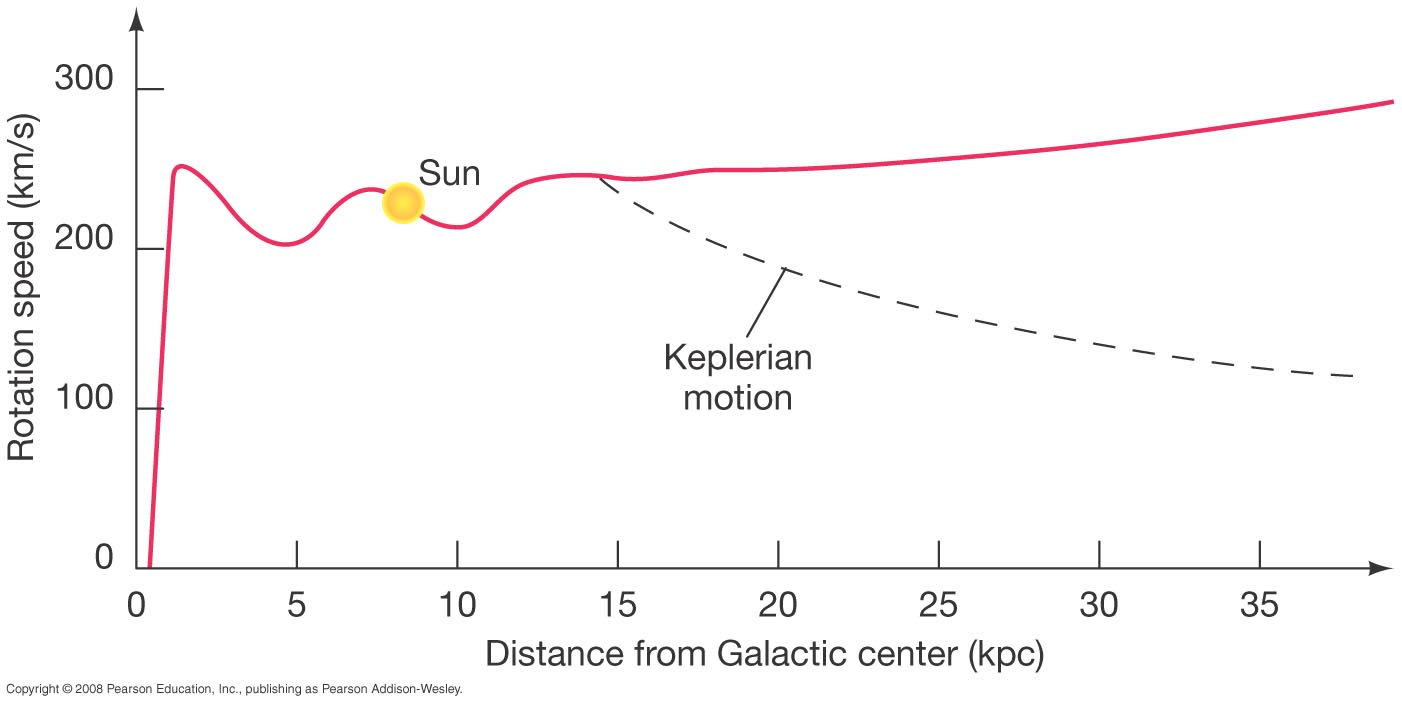
\includegraphics[width=0.7\textwidth]{Astrofysik/Astrofig/rotationskurve.jpg}
	\caption{Rotationskurve over Mælkevejen. Den solide kurve viser de observerede hastigheder, og den stiplede viser de forventede fra fordelingen af synligt stof. Afstanden mellem kurverne viser fordelingen af mørkt stof. Billede fra http://pages.uoregon.edu/jimbrau/BrauImNew/Chap23/6th/23\_21Figure-F.jpg
		}
	\label{rotationskurve}
\end{figure}

\subsection{Gravitationelle linser}

En af konsekvenserne af generel relativitetsteori er, at et massivt objekt kan fungere som en linse, der bøjer lyset fra en fjernere kilde. Fx kan lyset fra en kvasar blive bøjet af tyngdefeltet fra en galaksehob, der ligger mellem kilden og observatøren. Jo mere massiv en genstand er, jo større linseeffekt ser vi. Derfor kan vi fra effekten regne os frem til massen af det mellemliggende objekt. Hvis det er en galakse, kan vi se, at den bøjer rummet meget mere end hvad den burde ud fra det synlige lys. Igen mangler der altså masse, og mørkt stof må eksistere.


Stærk lensing er når forvrængningen af fx baggrundsgalakser, danner flere billeder af den samme galakse eller en hel ring rundt om det tunge objekt. Dette har vi observeret omkring mange fjerne hobe, hvilket inkluderer den berømte Abell 1689, se Figur \ref{abell1689}. Ved måling af forvrængningsgeometrien (Eng: distortion geometry) kan massen af den mellemliggende hob findes. %I mange tilfælde, hvor man har gjort dette, opnåede man masse-til-lys forhold svarende til det dynamiske mørke stof målt i hoben.

Svag gravitationel lensing undersøger små forvrængninger ved hjælp af statistiske analyser fra store galakseundersøgelser. Ved at undersøge den tilsyneladende forskydningsdeformation af de tilstødende baggrundsgalakser kan den gennemsnitlige fordeling af mørk stof karakteriseres.

Gravitationslinseeffekten kan også bruges til at opdage exoplaneter (planeter uden for Solsystemet). Det gælder, hvis lyset fra et objekt passerer en stjerne med en exoplanet, før det når frem til os. Så vil linsen forstærke lyset og vi ser et ekstra lille bump fra planetens tyngdekraft.

\begin{figure}[h!]
	\centering
	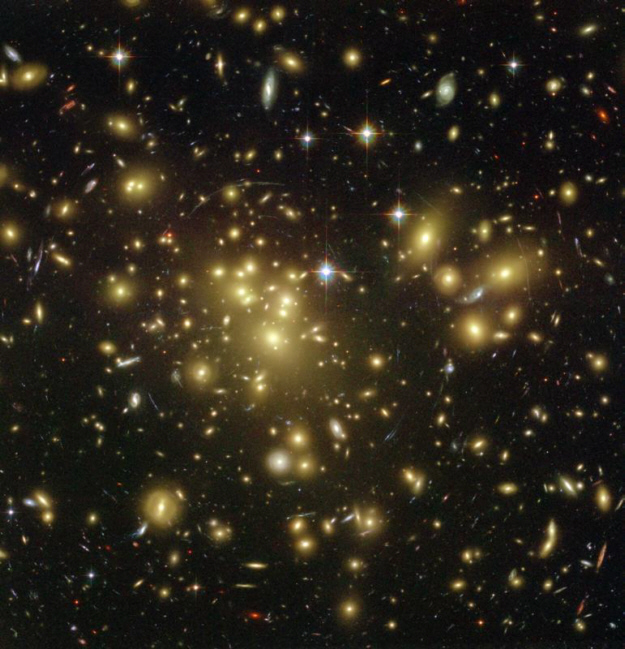
\includegraphics[width=0.6\textwidth]{Astrofysik/Astrofig/abell1689.jpg}
	\caption{Stærk gravitationel lensing observeret med Hubble Space Telescope, hvilket er en indikator for mørkt stof. Billede fra Hubble Space Telescope}
	\label{abell1689}
\end{figure}

\section{PERSPEKTIVERENDE}
Dette afsnit skal primært bruges, hvis vi har for lidt tekst og godt kunne tænke os at fylde den ud med noget perspektiverende 